\section{Numerical Studies of the Statistical Mechanisms}\label{sec:experiments}
The studies examine three distinct questions: how compatible learning
problems accumulate across lifetime scales, how the exploration clock
and capacity calibration affect finite-sample behavior, and how a
common reward environment interacts with a random schedule. All
reported losses are pseudo-regret relative to the best currently
available mean. The data are generated from the stated Bernoulli
models. Monte Carlo standard errors describe simulation uncertainty;
they are not uncertainty about a minimax constant.

\subsection{Risk on a Compatible Multiscale Family}\label{sec:geometry-experiment}
The first study evaluates the common null/spike family used in the lower-bound proof. At endpoint $T\in\{1024,4096,16384,65536\}$, batch $j$ has $2\cdot4^j$ competitors and lifetime $T/4^j$, for $j=0,\ldots,L-1$. We use $L\le3$ at the two smaller endpoints and $L\le4$ at the two larger ones. All groups survive the compatibility selection and contribute equally to the spectrum: $\cS_T=L\sqrt{2T}$ and $D_T^{\mathrm{eff}}=L$.

Each group has one reference arm. With probability $1/2$ all its candidates are below the reference; otherwise one uniformly selected candidate is above it. Independent configurations and deterministic increments in the reference means give one compatible stationary environment per replication. We use the proof's gap constant and the prespecified multipliers $a=4,8$, with $a=4$ in the main comparison. Larger multipliers preserve a legal prior but need not preserve the proof's total-variation bound. Each cell averages 128 independent draws of the environment and its Bernoulli observations. These finite-prior risks do not estimate the full minimax value.

For each multiscale schedule we construct a second schedule with the same endpoint and final number of arms: $2L$ competitors arrive at time one and the rest in the last round. The two fixed points differ by at most a factor $1.235$ in the simulated cases. At $T=65536$ and $L=4$, both equal 725, whereas the spectra are 1448.15 and 725.08. Under each schedule's native prior, MC-MOSS has mean regret 146.67 (Monte Carlo standard error 3.00) on the multiscale schedule and 87.57 (3.31) on the compressed schedule.

Because that comparison changes both schedule and prior, we also run each sampled mean vector on both schedules, using the same calendar reward uniforms. Compression reduces MC-MOSS regret by 18.82 (paired standard error 5.84) for the multiscale prior and by 185.04 (3.52) for the compressed prior. The difference separates the effect of arrival timing from the choice of a difficult environment.

Figure~\ref{fig:geometry-risk} reports the normalized losses and matched comparisons. At each fixed $L$, normalization by $\cS_T$ brings the endpoint curves close together, although the normalized risk still varies with $L$. Four effective scales do not demonstrate the asymptotic separation. In the largest four-scale case, the disjoint testing windows contribute 42.59 units of mean MC-MOSS regret, with 104.07 outside their union; the full loss enters every comparison. Cold MC improves on MC-MOSS under this native prior by 5.92 (paired standard error 1.38), but loses 40.44 (2.00) for the compressed prior run on the multiscale schedule. The finite-sample effect of retaining history depends on the environment.



For a six-environment prior at $T\in\{4,6,8,10\}$, exact dynamic programming gives a separate Bayes reference with known prior and schedule. At $T=8$, with gap increments $1/16$ and $1/8$, its risk is 0.289612, compared with 0.368656 for MC-MOSS and 0.431156 for Cold MC. The optimum is a certified lower bound for deterministic-schedule minimax risk, with more information than the anytime policies; the prior need not be least favorable. The computational supplement gives the recursion and its proof, all eight exact calculations, gap sensitivity, and individual window losses.

\begin{figure}[tbp]
 \centering
 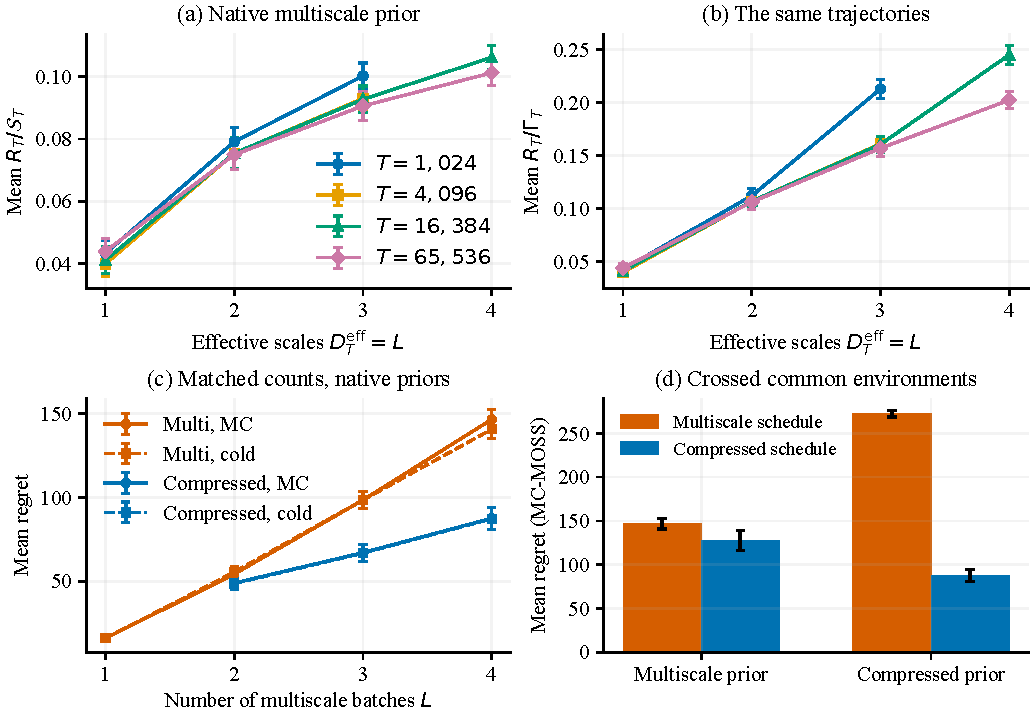
\includegraphics[width=\textwidth]{figures_v2/fig_geometry_risk.pdf}
 \caption{Bandit risk on a compatible finite product prior. Panels (a) and (b) use MC-MOSS and the native multiscale prior with gap multiplier four. Panel (c) compares each schedule under its native prior at $T=65536$; paired schedules have the same final count. Panel (d) fixes $T=65536$, $L=4$, and the sampled mean vector while changing its arrival schedule. Bars are $1.96$ Monte Carlo standard errors over 128 independent replications.}
 \label{fig:geometry-risk}
\end{figure}

\ifdefined\JASASubmission\FloatBarrier\fi
\subsection{Separating Clock Calibration, Capacity, and History}
\label{sec:mechanisms-experiments}

The next experiment separates the two changes hidden in a comparison with a
global-clock index.  We cross the clock, $s_t$ or $t$, with the capacity,
$d_j$ or $2(K_t-1)$, while retaining all observations in each of the four
rules.  Every rule uses the index
$\widehat\mu_i+\{\log_+(u_t/(v_tN_i))/N_i\}^{1/2}$, with the same
initialization and tie order.  MC-MOSS is the local-clock, frozen-capacity
cell.  A fifth rule uses precisely that cell but discards its observations
at the same capacity-doubling times.  These contrasts isolate finite-sample
effects; no spectral guarantee is asserted for the other three cells.

We also compare UCB1, AUER, Bernoulli KL-UCB, Thompson sampling, and clipped
MC-MOSS.  UCB1 and AUER use respective bonuses
$\{2\log(t)/N_i\}^{1/2}$ and $\{8\log(t)/N_i\}^{1/2}$
\citep{auer2002finite,kleinberg2008sleeping}.
KL-UCB uses the Bernoulli divergence and the original paper's recommended
experimental choice $c=0$ \citep{garivier2011kl}; Thompson sampling starts
each arriving arm with a $\operatorname{Beta}(1,1)$ prior
\citep{agrawal2012thompson}.  These are full-history arriving-arm
implementations of the stated rules.  We do not transfer their fixed-arm
guarantees to the present arrival model.

There are 32 candidates in batches of sizes $4,4,8,8,8$, arriving at
$1,\lfloor T/8\rfloor+1,\lfloor T/3\rfloor+1,
\lfloor T/2\rfloor+1,\lfloor3T/4\rfloor+1$, besides the initial anchor.
We fix five mean vectors: near ties, poor candidates, a persistent new
record at the fourth batch, a mixed-quality final batch, and an anchor at
the reward upper bound.  The full vectors are given in the supplement.
Both $T=2048$ and $T=8192$ are used.  Each cell has 128 independent
replications, coupled across methods by reward uniforms at each calendar
round.  We repeat the entire design with the order of labels reversed
within every candidate batch; the anchor remains first.  Parameters were
fixed before simulation, and software development used separate seeds.



Figure~\ref{fig:mechanisms-ablation} shows why the two factors must be
separated.  At $T=8192$, with forward labels and a mixed final batch, the
global clock costs $26.38$ (paired standard error $7.34$) relative to the
local clock when capacity is frozen.  With the global clock held fixed,
using current capacity reduces regret by $26.57$ ($1.30$).  The combined
global/current rule consequently has mean regret $224.24$, almost the
same as MC-MOSS's $224.42$, although the component contrasts are substantial.
Current capacity also improves on frozen capacity under the local clock,
by $18.90$ ($4.45$) in this example.  Thus the frozen capacity is a device
that supports the uniform analysis, not a claim of the best finite-sample
calibration.  Changing the clock to global increases mean regret in every
displayed cell, whereas discarding history is especially costly when
inferior candidates recur.  For poor candidates at $T=8192$, the latter
cost is $154.04$ ($2.12$).  Reversing labels preserves these broad patterns;
the near-tie differences at $T=2048$ are comparatively small and uncertain.

\begin{figure}[tbp]
\centering
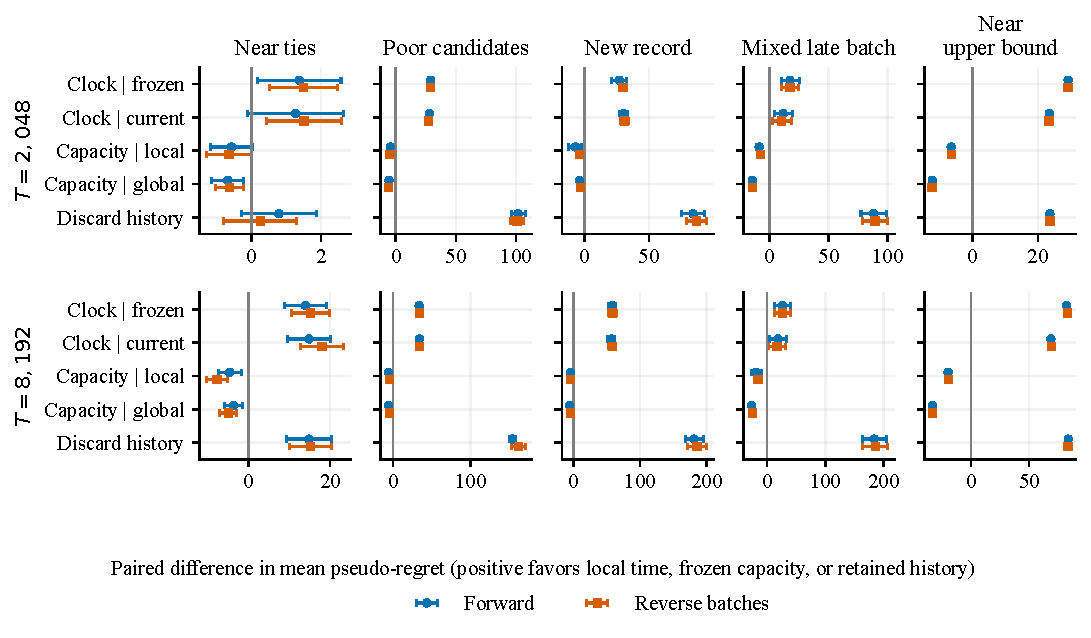
\includegraphics[width=\linewidth]{figures_v2/fig_mechanisms_ablation.pdf}
\caption{Matched mechanism contrasts under two horizons and two batch label
orders.  Clock contrasts are global minus local at fixed capacity;
capacity contrasts are current minus frozen at fixed clock.  Discarding
history is compared with MC-MOSS at identical reset times.  Points are
paired mean differences and bars are $1.96$ Monte Carlo standard errors
from 128 independent replications.  The intervals are pointwise, without
adjustment for the multiple displayed comparisons.  Horizontal scales
differ across panels.}
\label{fig:mechanisms-ablation}
\end{figure}

\begin{table}[t]
\centering
\caption{Pseudo-regret for four policies under five reward configurations.}
\label{tab:mechanisms-baselines}
\normalsize
\setlength{\tabcolsep}{3pt}
\begin{tabular*}{\linewidth}{@{\extracolsep{\fill}}lrrrr@{}}
\toprule
Configuration & MC-MOSS & KL-UCB & Thompson & Clipped MC \\
\midrule
Near ties & 103.85 (2.89) & 132.56 (0.50) & 125.81 (0.86) & 104.16 (2.69) \\
Poor candidates & 146.44 (0.86) & 236.00 (1.33) & 170.35 (1.12) & 147.36 (0.80) \\
New record & 157.11 (6.02) & 371.66 (3.06) & 242.72 (3.82) & 147.84 (4.55) \\
Mixed late batch & 224.42 (6.91) & 511.85 (5.57) & 304.10 (3.43) & 230.88 (7.33) \\
Near upper bound & 116.78 (0.36) & 1.70 (0.00) & 8.60 (0.30) & 0.00 (0.00) \\
\bottomrule
\end{tabular*}
\par\medskip\noindent\begin{minipage}{\linewidth}\normalsize\setstretch{1}
\textit{Notes:} Entries are mean pseudo-regret with Monte Carlo standard errors in parentheses at $T=8192$, forward labels, and 128 replications. The complete two-horizon, two-label-order results, including UCB1 and AUER, are in the computational supplement and released CSV files.
\end{minipage}
\end{table}


The stronger baselines also identify a substantial failure of the
unclipped rule (Table~\ref{tab:mechanisms-baselines}).  With anchor mean one
and candidate means $0.94$ or $0.985$, MC-MOSS incurs $116.78$ mean regret
at $T=8192$, compared with $1.70$ for KL-UCB and $8.60$ for Thompson sampling.
Clipped MC-MOSS has zero regret here: its indices never exceed one and
the specified tie rule keeps selecting the anchor.  This conclusion uses
the exact boundary mean and the anchor's priority; it is not an assertion
of uniform dominance by clipping.  Indeed, in the mixed-final-batch
configuration clipping changes regret by $6.46$ ($8.76$), with no resolved
improvement.  The comparisons support the roles of clock calibration and
history reuse while showing that a minimax guarantee leaves room for
large improvements on particular reward distributions.

\ifdefined\JASASubmission\FloatBarrier\fi
\subsection{A Common Environment Across Random Arrival Scales}\label{sec:experiment-random}
The third study holds the two reward means fixed before drawing the
arrival schedule. At $T=4^m$, $m=4,5,6,7$, the competing arm has lifetime
$H=4^J$, $J=0,\ldots,m$. We consider probabilities proportional to
$2^{-J}$, uniform scale probabilities, probabilities proportional to
$4^{-J}$, an equal mixture of the last two scales, and a point mass at
the last scale. The anchor mean is $1/2$; the competitor mean is
$1/2\pm\Delta$, with $\Delta=2^{-1-r/2}$, $r=0,\ldots,2m+2$.

One rule starts a fresh two-arm MOSS run with the remaining horizon
revealed by the known endpoint. The other is the original MC-MOSS,
which does not know the endpoint and retains all anchor observations.
Their panels specify this information difference. We simulate the
forced prefix exactly through its binomial sufficient statistic.

For each policy and mixture, we use 64 development replications to
select a single gap and sign, or a separate gap and sign for each lifetime.
Both selections are then evaluated on 128 independent replications per
lifetime. Mixture means use the known schedule probabilities, with
stratified Monte Carlo standard errors. A separate check draws 2048
actual schedules for each selected common environment. These are
held-out risks of development-selected members of a finite grid, not
estimates of the full minimax risk or of a continuous supremum.

Figure~\ref{fig:random-heatmap} shows the conditional risk of a better
arriving competitor. The difficult gap changes with the remaining
lifetime. The retained prefix changes this surface, so the two panels
also differ for reasons beyond endpoint information alone.
Figure~\ref{fig:random-common} then averages over the inverse-square-root
mixture. At the largest endpoint, fresh-horizon MOSS has held-out mean
regret 1.321 (standard error 0.018) under the selected common
environment, compared with 1.977 (0.026) when the selected
environment is allowed to depend on the schedule. The corresponding
geometric values are $W(Q)=1.412$ and $\mathbb E\sqrt H=4.016$.
The latter curve is an arrival-only reference, not an observed risk.

The remaining mixtures, direct schedule draws and selected gaps are
reported in the computational supplement. For the two-long-scale
mixture the held-out ordering is reversed: development selection can
miss the best grid member. Independent evaluation removes reuse of
selection noise from the reported means; it does not make finite-grid
selection exact. None of these finite experiments estimates an
asymptotic rate or establishes that the anytime policy attains the
random-template theorem.

\begin{figure}[tbp]
\centering
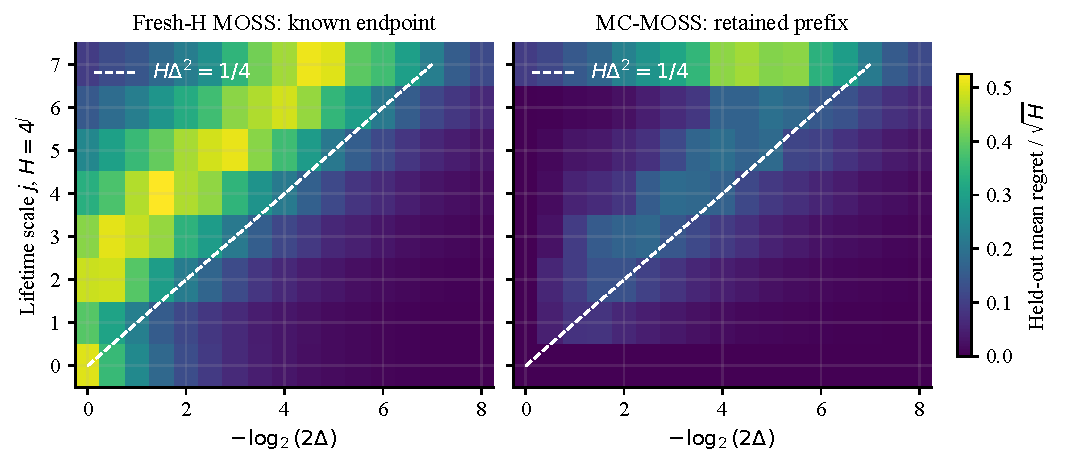
\includegraphics[width=\textwidth]{figures_v2/random_gap_heatmap.pdf}
\caption{Held-out regret divided by $\sqrt H$ for a better arriving
competitor at $T=16384$. Each cell uses 128 replications. The dashed
line marks $H\Delta^2=1/4$; it is a scale reference, not a fitted ridge.
The policies differ in endpoint knowledge and retention of the forced
anchor prefix.}\label{fig:random-heatmap}
\end{figure}
\begin{figure}[tbp]
\centering
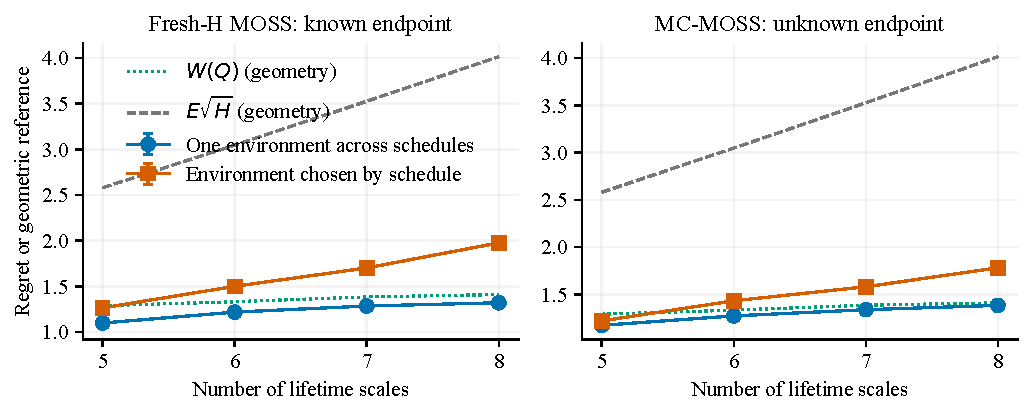
\includegraphics[width=\textwidth]{figures_v2/random_common_gap.pdf}
\caption{Common versus schedule-specific environments under
$\Pr(J=j)\propto2^{-j}$. Environments are selected on development
replications and evaluated independently. Bars are 1.96 stratified
Monte Carlo standard errors. The two geometric reference curves are
computed from the arrival law and are not risk estimates. Selection
is performed separately for each policy; the panels do not compare
the policies under one common mean vector.}
\label{fig:random-common}
\end{figure}

\ifdefined\JASASubmission\FloatBarrier\fi
\subsection{Two Fixed Batches Under a Random Common Stretch}
\label{sec:stretch-experiment}

We finally check the executable upper-bound construction on a template
with two batches of two candidates, $\boldsymbol\alpha=(4,1)$ and $K=5$.
Let $T=4\cdot4^m$, $m=3,4,5,6$, and let $H$ range over
$1,4,\ldots,4^m$.  We consider the inverse-square-root law
$\PP(H=4^j)\propto2^{-j}$, the uniform law on these scales, and the
deterministic longest scale.  Once the first batch arrives, the rule in
Theorem~\ref{thm:random-positive-main} runs fresh fixed-horizon MOSS experiments
of lengths $3H$ and $H$.  The comparison is the original anytime MC-MOSS,
which retains all observations, including the anchor's prefix.  The
former rule uses the known endpoint and revealed schedule; MC-MOSS is
given neither.

The fixed reward vector is
$(0.50,0.45,0.55,0.55+\eta\delta,0.50)$, with
$\eta\in\{-1,1\}$ and
$\delta\in\{0.025,0.05,0.10,0.20,0.40\}$.
For each $(m,Q)$ we use 64 development replications to select the single
pair $(\eta,\delta)$ with the largest law-averaged regret for the
revealed-stretch rule.  We evaluate that same pair on 128 independent
held-out replications for both policies and every value of $H$.
Thus no environment is selected after the realized stretch.  The finite
law is averaged exactly over its support, with Monte Carlo sampling only
for rewards.  These are held-out risks for selected common environments,
not estimates of the continuous minimax supremum.



At $m=6$, the inverse-square-root law has $W(Q)=1.386$;
the revealed-stretch rule has mean regret $5.94$ (standard error $0.05$),
and MC-MOSS has $3.11$ ($0.06$).  The corresponding revealed-stretch risks
are $39.81$ ($0.58$) under the uniform-scale law and $141.80$ ($3.14$)
under the deterministic longest scale, whose complexities are $12.190$
and $64$, respectively.  Figure~\ref{fig:stretch-heldout} displays the
normalized values across all four endpoints.  MC-MOSS performs better
in every selected cell, despite using less schedule information.  This
does not contradict the theorem: the reset construction proves an
upper bound and is not optimized for finite-sample constants.  Nor does
this finite grid establish the asymptotic rate or a matching lower
constant.  Its role is to verify that the common-environment averaging
and the multi-batch upper-bound rule can be implemented without
discarding regret incurred before the last batch.


\begin{figure}[tbp]
\centering
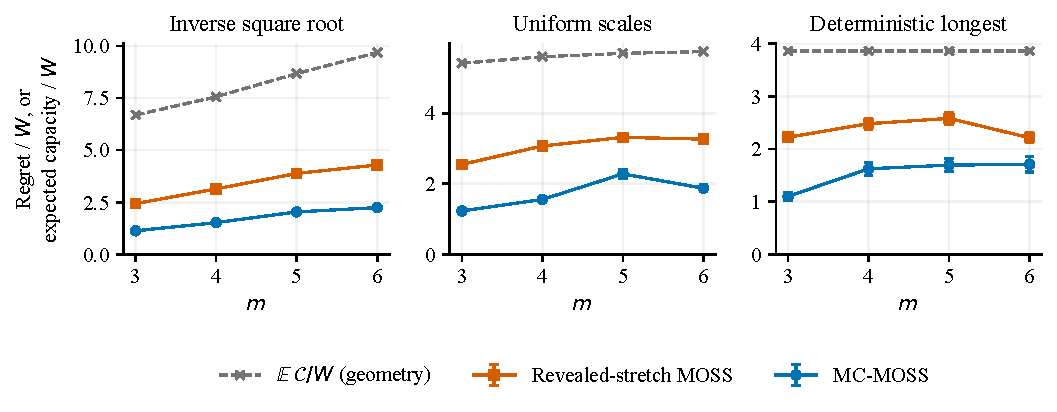
\includegraphics[width=\linewidth]{figures_v2/fig_stretch_heldout.pdf}
\caption{Held-out common-environment risks divided by $W(Q)$ for the
fixed two-batch template.  Error bars are $1.96$ Monte Carlo standard
errors under exact stratification over $H$.  The dashed curve is the
expected deterministic capacity divided by $W(Q)$ and is a geometric
reference, not an observed regret.  Both policies face the same
development-selected environment in each panel and at each $m$.}
\label{fig:stretch-heldout}
\end{figure}
\ifdefined\JASASubmission\FloatBarrier\fi
